A representação do quadricóptero criada no Simulink\textsuperscript{\textregistered} seguindo a modelagem de \citeonline{Balas2007} é mostrada na Figura \ref{fig:diagram_drone_block}. 

\begin{figure}[!htb]
    \centering
    \caption{Representação do quadricóptero no \textit{Simulink}}
    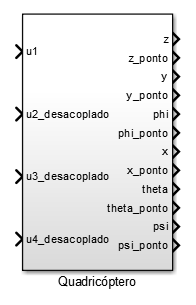
\includegraphics[width=0.3\textwidth]{./04-figuras/figuras_pos_banca/1-mostrando_desacoplamento/diagram_drone_block}
    \label{fig:diagram_drone_block}
\end{figure}
Como se pode ver, o sistema inclui os quatro sinais de entrada seguindo o desacoplamento desenvolvido (\textit{u1}, \textit{u2\_desacoplado}, \textit{u3\_desacoplado} e \textit{u4\_desacoplado}) e com as doze saídas referentes às seis variáveis de configuração $x$ ,$y$, $z$, $\phi$, $\theta$, $\psi$ indicadas por x, y, z, phi, theta e psi, respectivamente; e suas respectivas variações $\dot{x}$ ,$\dot{y}$, $\dot{z}$, $\dot{\phi}$, $\dot{\theta}$, $\dot{\psi}$ representadas por x\_ponto, y\_ponto, z\_ponto, phi\_ponto, theta\_ponto e psi\_ponto.

Para mostrar o desacoplamento das variáveis, alternadamente foi aplicado um sinal de degrau a cada uma das entradas. Em cada um dos casos, somente uma entrada era submetida ao degrau, ao passo que as demais eram aterradas. As respostas, a cada um dos experimentos, das variáveis de configuração relativas à altitude e atitude do quadricóptero são mostradas nas Figuras \ref{fig:graphs_step_u1}, \ref{fig:graphs_step_u2}, \ref{fig:graphs_step_u3} e \ref{fig:graphs_step_u4} tomando como estado inicial um quadricóptero estável ($\phi$ = $\theta$ = $\psi$ = 0 rad) a trinta metros de altura ($z$ = 30 m).

\begin{figure}[!htb]
    \centering
    \caption{Resposta das saídas z, $\phi$, $\theta$ e $\psi$ a um entrada em degrau em $u1$}
    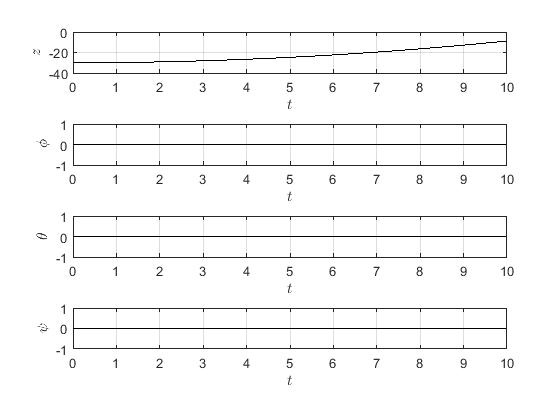
\includegraphics[width=0.8\textwidth]{./04-figuras/figuras_pos_banca/1-mostrando_desacoplamento/graphs_step_u1}
    \label{fig:graphs_step_u1}
\end{figure}

\begin{figure}[!htb]
    \centering
    \caption{Resposta das saídas z, $\phi$, $\theta$ e $\psi$ a um entrada em degrau em $u2\_desacoplado$}
    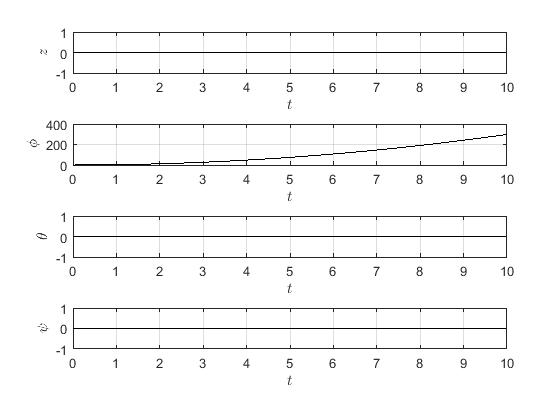
\includegraphics[width=0.8\textwidth]{./04-figuras/figuras_pos_banca/1-mostrando_desacoplamento/graphs_step_u2}
    \label{fig:graphs_step_u2}
\end{figure}

\begin{figure}[!htb]
    \centering
    \caption{Resposta das saídas z, $\phi$, $\theta$ e $\psi$ a um entrada em degrau em $u3\_desacoplado$}
    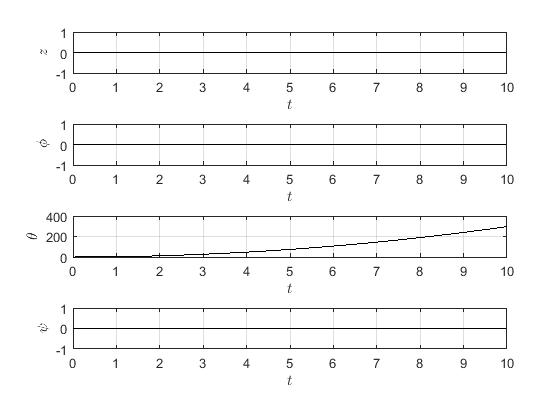
\includegraphics[width=0.8\textwidth]{./04-figuras/figuras_pos_banca/1-mostrando_desacoplamento/graphs_step_u3}
    \label{fig:graphs_step_u3}
\end{figure}

\begin{figure}[!htb]
    \centering
    \caption{Resposta das saídas z, $\phi$, $\theta$ e $\psi$ a um entrada em degrau em $u4\_desacoplado$}
    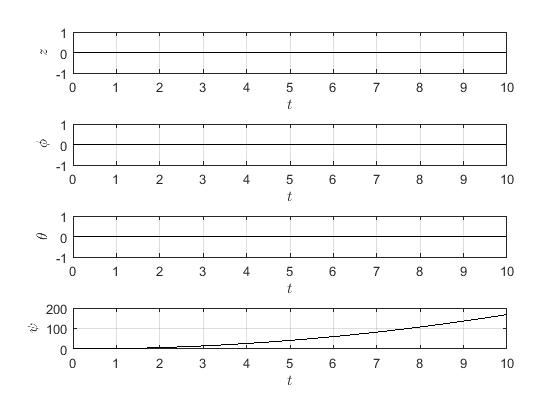
\includegraphics[width=0.8\textwidth]{./04-figuras/figuras_pos_banca/1-mostrando_desacoplamento/graphs_step_u4}
    \label{fig:graphs_step_u4}
\end{figure}

Como se pode ver, cada entrada afeta uma única saída e cada saída é afetada apenas por uma entrada. Com isso, mostra-se o desacoplamento existente que faz com que a entrada $u1$ somente interfira na variável de configuração $z$; $u2\_desacoplado$ em $\phi$; $u3\_desacoplado$ em $\theta$; e $u4\_desacoplado$ em $\phi$.
